\documentclass{article}
\usepackage[utf8]{inputenc}
\usepackage{caption}
\usepackage[margin=1in]{geometry}
\usepackage{graphicx}
\title{System Requirements Specification}
\author{Team EVAL}
\date{October 29, 2018}

\begin{document}

\maketitle

\newpage

\begin{center}
{
\includegraphics[scale=.3]{images/team_logo.png}}\\ \bigskip
{\LARGE College Course Evaluation System }\\ \medskip
{\large System Requirements Specification }\\ \medskip
\end{center}

\tableofcontents

\newpage

\section{Introduction}
\subsection{Purpose of this Document}

This system requirements specification details what our course evaluation system does and what tests we will make to ensure the system is complete. It includes why we are creating the system, the scope of the product, diagrams that illustrate the system, what we will deliver to the customer, and currently pending issues about the software.

This document is intended for the development team, the product client, Dr. Harlan Onsrud, and potential users of the system. Team EVAL needs this document to ensure that the product works as intended. Dr. Onsrud needs it to know that he will receive the program that he desires. The document also helps the software's users in that they can learn more about the functions of the evaluation system.

\subsection{References}

LimeSurvey: The online survey tool - open source surveys. (n.d.). Retrieved from

https://www.limesurvey.org/

\medskip \noindent
Fowler, M. (2004). UML Distilled: A Brief Guide to the Standard Object Modeling Language. Boston:

Addison-Wesley.

\subsection{Purpose of the Product}

The University of Maine gives out course evaluation surveys to students at the end of each course. The survey is filled on a bubble sheet and is then scanned. Harlan Onsrud finds it inconvenient for the school administrators to manually scan and compile the survey results. Current campus experiments with electronic evaluations are not fully automated and do not seem to fulfill the desires of students and faculty. He desires an online, automated evaluation system that is responsive to the University's community needs and improves productivity.\par

\subsection{Product Scope}

Team EVAL will create a product which interfaces with an already existing survey software, LimeSurvey, to provide both individual teachers and administrators the ability to create and administer evaluations.  This product will be usable even by those without technical backgrounds, and it will have an intuitive interface for setting up and administering teacher evaluations.

It will allow users to create one or more courses with predefined survey data and rosters of e-mail addresses.  For each class, users will be able to choose from provided questions or enter their own custom questions.  The question sets that they make may be saved to their account and applied to future evaluations they create.  Upon request of the user, the product will create a LimeSurvey with the supplied information. It then sends an invitation to complete the survey to the students on the class' roster via e-mail, along with reminders as appropriate.  When the survey is terminated by the instructor/administrator or by a certain data and time, the product will allow users to view and download a statistical analysis and clear visualization of the data collected for one or more of their courses.

The software will support the reporting of accumulated data and the appropriate statistics and graphics derived from it for each academic period. A report will be generated for the following levels: course section, all sections of the same course, all courses of each instructor, all courses with the same designator (e.g. ``COS''), all courses in the same department/school, all courses in the same college, and all courses in the same university.

The product will be completed in time to administer teacher evaluations for the spring of 2019 at the University of Maine, whether evaluation forms are created by instructors or administrators. A UML diagram (Figure 1) shows the scope as a dotted rectangle.

LimeSurvey is an existing software that has the ability to create and publish surveys. This product will simply interface with LimeSurvey and interact with its components. LimeSurvey lies outside of the scope of this project and will be treated as a third party actor.\par

\begin{center}
\begin{figure}
    \centering
    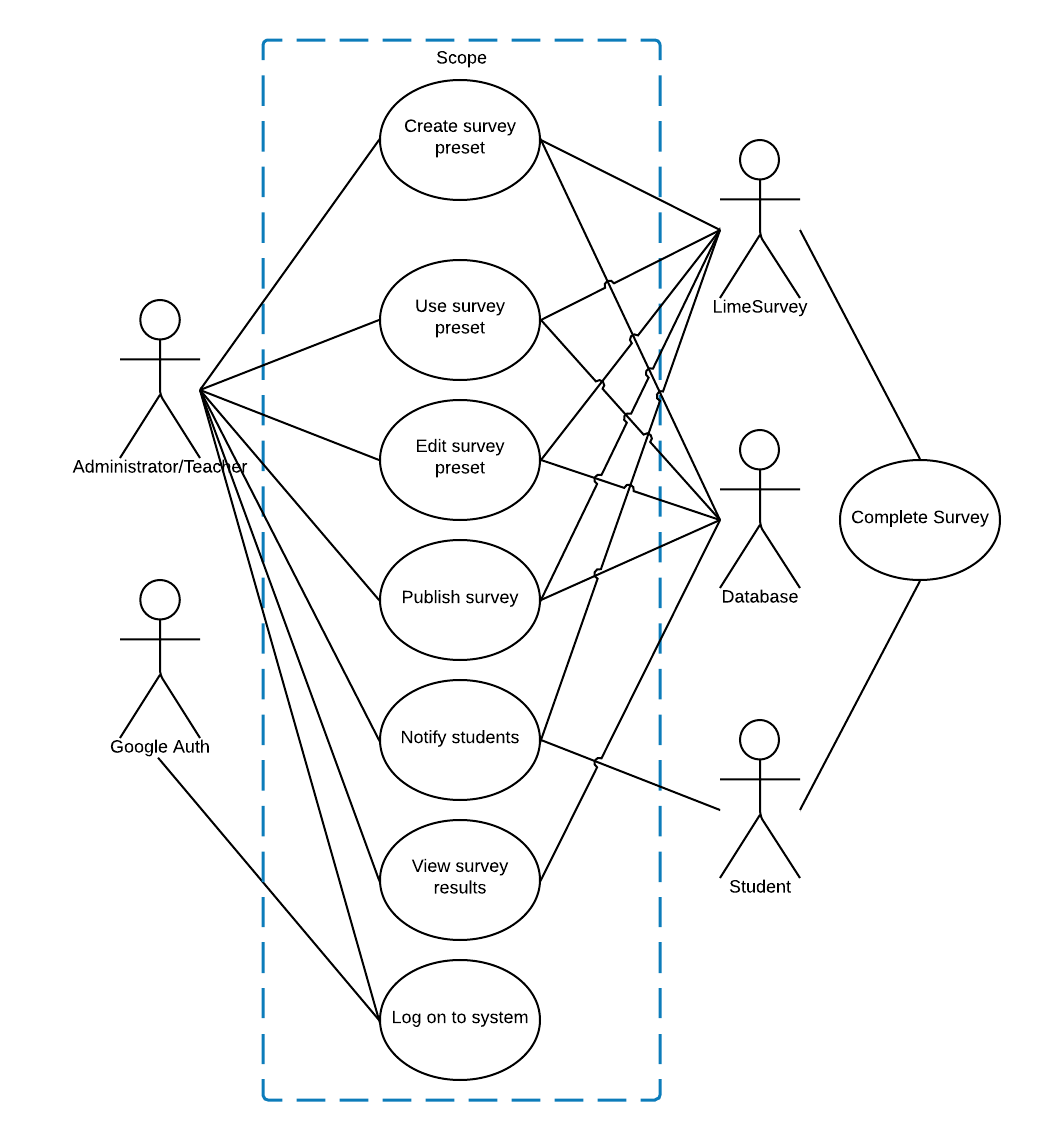
\includegraphics[scale=.75]{images/scope_diagram.png}
    \caption{Use Case diagram of the system scope.}
    \label{fig:my_label}
\end{figure}
\end{center}

\newpage

\section{Functional Requirements}

The functional requirements specify what actions the program will perform. Each requirement is represented as a use case. The UML diagram showing the use cases is on the next page.

\begin{center}

\captionof{table}{}
\begin{tabular}{|p{3.5cm}|p{7.5cm}|} 
\hline
\textbf{Number} & 1 \\
\hline
\textbf{Name} & Log on to system  \\ 
\hline
\textbf{Summary} & A teacher or administrator logs in with a username and password \\ 
\hline
\textbf{Priority} & 5\\ 
\hline
\textbf{Preconditions }& The user has an Google account (or can otherwise sign in with Google) \\ 
\hline
\textbf{Postconditions} & A session is started and an authentication token is sent to the program \\ 
\hline
\textbf{Primary Actors }& Administrator, Teacher\\ 
\hline
\textbf{Secondary Actors} & Google Authentication \\ 
\hline
\textbf{Trigger }& A user attempts to log in \\ 
\hline
\textbf{Main Scenario }& 
\begin{tabular}{l|p{5.8cm}} 
\textbf{Step }& \textbf{Action}\\
\hline
1 & Open the log-in page \\
\hline
2 & Enter Google log-in information \\
\hline
3 & User is authenticated \\
\hline
4 & User gains access to the system\\
\end{tabular}\\ 
\hline
\textbf{Extensions }&
\begin{tabular}{l|p{5.8cm}} 
\textbf{Step }& \textbf{Branching Action}\\
\hline
2a & Incorrect log-in info : Do not proceed and alert user  \\
\end{tabular}\\
\hline
\textbf{Open Issues} & What method to use for authentication of non-anonymous comments by students \\     
\hline
\end{tabular}

\bigskip
\captionof{table}{}
\begin{tabular}{|p{3.5cm}|p{7.5cm}|} 
\hline
\textbf{Number} & 2  \\
\hline
\textbf{Name} & Create survey preset  \\ 
\hline
\textbf{Summary} & An administrator or teacher adds a preset list of questions to the database \\ 
\hline
\textbf{Priority} & 5\\ 
\hline
\textbf{Preconditions }& A course's evaluation survey questions are unchosen or unwritten \\ 
\hline
\textbf{Postconditions} & The course's evaluation survey is written \\ 
\hline
\textbf{Primary Actors }& Administrator, Teacher \\ 
\hline
\textbf{Secondary Actors} & Database, LimeSurvey \\ 
\hline
\textbf{Trigger }& A new course needs to be evaluated \\ 
\hline
\textbf{Main Scenario }& 
\begin{tabular}{l|p{5.8cm}} 
\textbf{Step }& \textbf{Action}\\
\hline
1 & Select option to add a preset \\
\hline
2 & Enter the survey data on LimeSurvey\\
\hline
3 & Database updated with survey info\\
\end{tabular}\\ 
\hline
\textbf{Extensions }&
\begin{tabular}{l|p{5.8cm}} 
\textbf{Step }& \textbf{Branching Action}\\
\hline
2a & Invalid data is entered : Notify user of incorrect data  \\
\end{tabular}\\
\hline
\textbf{Open Issues} & What information about the survey shall be stored, what format should the data be in\\ 
\hline
\end{tabular}

\bigskip
\vspace{1.5in}
\captionof{table}{}
\begin{tabular}{|p{3.5cm}|p{7.5cm}|} 
\hline
\textbf{Number} & 3  \\
\hline
\textbf{Name} & Use survey preset \\ 
\hline
\textbf{Summary} & An administrator or teacher retrieves a preset for a survey developed previously for a course\\
\hline
\textbf{Priority} & 4\\ 
\hline
\textbf{Preconditions }& The survey preset exists in the database \\ 
\hline
\textbf{Postconditions} & A preset list is available to create a survey \\ 
\hline
\textbf{Primary Actors }& Administrator, Teacher \\ 
\hline
\textbf{Secondary Actors} & Database, LimeSurvey \\ 
\hline
\textbf{Trigger }& A user wants the same questions as on a previous survey \\ 
\hline
\textbf{Main Scenario }& 
\begin{tabular}{l|p{5.8cm}} 
\textbf{Step }& \textbf{Action}\\
\hline
1 & Select option to use a preset list of questions \\
\hline
2 & Choose which preset to use\\
\hline
3 & Preset data from database converted to LimeSurvey form\\
\hline
4 & LimeSurvey updated with preset\\
\end{tabular}\\ 
\hline
\textbf{Extensions }&
\begin{tabular}{l|p{5.8cm}} 
\textbf{Step }& \textbf{Branching Action}\\
\hline
2a & Data in preset is invalid : Notify user of invalid data  \\
\end{tabular}\\
\hline
\textbf{Open Issues} & Which presets are visible to each teacher \\ 
\hline
\end{tabular}

\bigskip
\captionof{table}{}
\begin{tabular}{|p{3.5cm}|p{7.5cm}|} 
\hline
\textbf{Number} & 4  \\
\hline
\textbf{Name} & Edit survey preset  \\ 
\hline
\textbf{Summary} & An administrator or teacher edits the survey questions for a course \\ 
\hline
\textbf{Priority} & 5\\ 
\hline
\textbf{Preconditions }& A course for the survey questions exists in the database \\ 
\hline
\textbf{Postconditions} & A course includes appropriate survey data \\ 
\hline
\textbf{Primary Actors }& Administrator, Teacher \\ 
\hline
\textbf{Secondary Actors} & Database, LimeSurvey \\ 
\hline
\textbf{Trigger }& A college course survey has incorrect data or preferences \\ 
\hline
\textbf{Main Scenario }& 
\begin{tabular}{l|p{5.8cm}} 
\textbf{Step }& \textbf{Action}\\
\hline
1 & Choose the course whose questions are to be edited \\
\hline
2 & Select questions preset if applicable\\
\hline
3 & Modify the data to be appropriate for the course\\
\hline
4 & Database updated with new edits\\
\end{tabular}\\ 
\hline
\textbf{Extensions }&
\begin{tabular}{l|p{5.8cm}} 
\textbf{Step }& \textbf{Branching Action}\\
\hline
3a & Invalid data is entered : Notify user of incorrect data  \\
\end{tabular}\\
\hline
\textbf{Open Issues} & None \\ 
\hline
\end{tabular}

\vspace{4in}
\captionof{table}{}
\begin{tabular}{|p{3.5cm}|p{7.5cm}|} 
\hline
\textbf{Number} & 5  \\
\hline
\textbf{Name} & Publish survey  \\ 
\hline
\textbf{Summary} & LimeSurvey or the evaluation software is used to send out a survey to students \\ 
\hline
\textbf{Priority} & 5\\ 
\hline
\textbf{Preconditions }& The chosen class has questions entered \\ 
\hline
\textbf{Postconditions} & A survey is created using LimeSurvey and sent to the students on the class roster \\ 
\hline
\textbf{Primary Actors }& Administrator, Teacher \\ 
\hline
\textbf{Secondary Actors} & Database, LimeSurvey\\ 
\hline
\textbf{Trigger }& A teacher or administrator wants to send out an evaluation \\ 
\hline
\textbf{Main Scenario }& 
\begin{tabular}{l|p{5.8cm}} 
\textbf{Step }& \textbf{Action}\\
\hline
1 & Select option to publish survey \\
\hline
2 & Select course(s)\\
\hline
3 & A survey is created using LimeSurvey\\
\hline
4 & The survey is sent to all students on the class roster\\
\end{tabular}\\ 
\hline
\textbf{Open Issues} & None\\ 
\hline
\end{tabular}

\bigskip
\captionof{table}{}
\begin{tabular}{|p{3.5cm}|p{7.5cm}|} 
\hline
\textbf{Number} & 6  \\
\hline
\textbf{Name} & Notify students  \\ 
\hline
\textbf{Summary} & LimeSurvey or the evaluation software is used to e-mail students to complete the survey, giving up to 3 automatic reminders as appropriate \\ 
\hline
\textbf{Priority} & 5\\ 
\hline
\textbf{Preconditions }& A course evaluation survey is completed \\ 
\hline
\textbf{Postconditions} & All students are finished with their survey, or a deadline is reached\\ 
\hline
\textbf{Primary Actors }& Teacher \\ 
\hline
\textbf{Secondary Actors} & Student, LimeSurvey \\ 
\hline
\textbf{Trigger }& The teacher releases the survey to students \\ 
\hline
\textbf{Main Scenario }& 
\begin{tabular}{l|p{5.8cm}} 
\textbf{Step }& \textbf{Action}\\
\hline
1 & Send initial reminder to students \newline about survey using course roster\\
\hline
2 & Students complete survey\\
\hline
3 & Copy LimeSurvey results to database\\
\hline
4 & Database deletes data that is 60 days old\\
\end{tabular}\\ 
\hline
\textbf{Extensions }&
\begin{tabular}{l|p{5.8cm}} 
\textbf{Step }& \textbf{Branching Action}\\
\hline
2a & A student does not complete survey  : Send another reminder to student  \\
\end{tabular}\\
\hline
\textbf{Open Issues} & How often to remind students, how to handle signed comments \\ 
\hline
\end{tabular}

\bigskip
\vspace{2.6in}
\captionof{table}{}
\begin{tabular}{|p{3.5cm}|p{7.5cm}|} 
\hline
\textbf{Number} & 7 \\
\hline
\textbf{Name} & View survey results  \\ 
\hline
\textbf{Summary} & An administrator, teacher, or both receive an automated e-mail, which has a link to view or download the survey results (i.e. averages and charts) \\ 
\hline
\textbf{Priority} & 4\\ 
\hline
\textbf{Preconditions }& Survey responses are entered in database \\ 
\hline
\textbf{Postconditions} & All appropriate averages are computed and displayed \\ 
\hline
\textbf{Primary Actors }& Administrator, Teacher \\ 
\hline
\textbf{Secondary Actors} & Database \\ 
\hline
\textbf{Trigger }& A user seeks information about the responses to a group of surveys \\ 
\hline
\textbf{Main Scenario }& 
\begin{tabular}{l|p{5.8cm}} 
\textbf{Step }& \textbf{Action}\\
\hline
1 & Click link to view results \\
\hline
2 & Compute average score for each question \\
\hline
3 & Display results by instructor, department, and university \\
\hline
4 & Select option to download results\\
\end{tabular}\\ 
\hline
\textbf{Open Issues} & Which survey questions are averaged for display \\ 
\hline
\end{tabular}
\end{center}


\newpage

\subsection{Tests}

These are the tests that will verify the functional requirements:

\begin{enumerate}
  \item (Use Case 1) The tester attempts to log on to the system using four different sets of credentials: a valid e-mail address and password of an existing account (with courses already created), a valid address and password of a nonexistent account, an address with an invalid password for an existing account, and an invalid e-mail address and password. The test is successful if the first set passes and the last three sets fail. In the second case, a user will be prompted to register for the system. 
  \item (Use Case 2) The tester selects the option to add a course preset, then submits evaluation questions, preferences, the course roll, and e-mail texts. The test is successful only if all the data entered is reflected in the database.  The data should still be there after logging out of the system. The team will create several courses/sections of the same course to ensure that the data loaded into LimeSurvey remains unchanged from when the original course was loaded. We will test adding students' full names and e-mails to the list of enrolled students.
  \item (Use Case 3) The tester creates a course survey. He or she then tries to select that same survey to be used again. The new preset should still be present on LimeSurvey. The test is successful only if the preset data is loaded correctly to LimeSurvey from the database. The tester will exit the evaluation system and log in again to ensure that the data is saved.
  \item (Use Case 4) The tester selects the option to create a survey. Next, he or she chooses a questions preset for the survey. The tester then adds one question and edits an existing question from the preset. After submitting, the database should include the new survey, containing the preset list, added question, and edited question. The team will run the program several times, each time selecting different questions to be included in the survey. We will ensure that some questions are mandatory and must be included no matter what.
  \item (Use Case 5) The tester creates a course survey, does not enter any questions, and attempts to send the survey.  The tester then enters some questions and sends the survey again.  The team verifies that the survey is created with all questions entered and that the e-mail addresses on the course roster receive a prompt to complete it. 
  \item (Use Case 6) The tester messages a group of ten unique people about a mock survey. In a successful test, all ten people receive an e-mail with each containing a link to the survey. Most respondents promptly complete the survey, but one does not. The database must contain the survey responses of the nine people who finished, and the program must send another reminder e-mail to the unfinished person about the survey. Finally, the database must delete old survey data. The team will set the time periods before the reminder e-mail and data deletion to be very short to test whether the two functions work.
  \item (Use Case 7) The tester selects the option to view the survey results. There are survey results using mock data for (a) each course section, (b) all sections of the same course, (c) all courses of each instructor, (d) all courses with the same designator, (e) all courses in the same department/school, (f) all courses in the same college, and (g) all courses in the same university. The team will add several surveys, each with different questions. If the test is successful, the correct average scores for every question in the course evaluation survey are shown in the application. Bar graphs for each course and section are supplied as well. Also, the software must show the appropriate results for all seven levels listed above.
\end{enumerate}

\newpage
\section{Non-Functional Requirements}

The non-functional requirements state the qualities of the program that are unrelated to its function.

\begin{center}
\captionof{table}{}
\begin{tabular}{|p{3.5cm}|p{7.5cm}|} 
\hline
\textbf{Number} & 1  \\
\hline
\textbf{Priority} & 3\\ 
\hline
\textbf{Description} & The software should be supported by the latest versions of Windows, Mac, Linux, iOS, and Android. \\ 
\hline
\textbf{Test Number(s) }& 1 \\ 
\hline
\end{tabular}

\bigskip
\captionof{table}{}
\begin{tabular}{|p{3.5cm}|p{7.5cm}|} 
\hline
\textbf{Number} & 2  \\
\hline
\textbf{Priority} & 4\\ 
\hline
\textbf{Description} & The software should be accessible by the latest versions of Safari, Chrome, Firefox, and Edge. \\ 
\hline
\textbf{Test Number(s) }& 2 \\ 
\hline
\end{tabular}


\bigskip
\captionof{table}{}
\begin{tabular}{|p{3.5cm}|p{7.5cm}|} 
\hline
\textbf{Number} & 3  \\
\hline
\textbf{Priority} & 5\\ 
\hline
\textbf{Description} & All questions entered by the teacher or administrator shall appear on the output survey. \\ 
\hline
\textbf{Test Number(s) }& 3 \\ 
\hline
\end{tabular}


\bigskip
\captionof{table}{}
\begin{tabular}{|p{3.5cm}|p{7.5cm}|} 
\hline
\textbf{Number} & 4  \\
\hline
\textbf{Priority} & 5\\ 
\hline
\textbf{Description} & All data stored in the program's database shall be valid. \\ 
\hline
\textbf{Test Number(s) }& 4 \\ 
\hline
\end{tabular}


\bigskip
\captionof{table}{}
\begin{tabular}{|p{3.5cm}|p{7.5cm}|} 
\hline
\textbf{Number} & 5  \\
\hline
\textbf{Priority} & 5\\ 
\hline
\textbf{Description} & All collected survey data shall not be alterable.\\ 
\hline
\textbf{Test Number(s) }& 5 \\ 
\hline
\end{tabular}


\bigskip
\captionof{table}{}
\begin{tabular}{|p{3.5cm}|p{7.5cm}|} 
\hline
\textbf{Number} & 6  \\
\hline
\textbf{Priority} & 4\\ 
\hline
\textbf{Description} & Teachers shall not be able to access data of courses other than their own. \\ 
\hline
\textbf{Test Number(s) }& 6 \\ 
\hline
\end{tabular}


\bigskip
\vspace{1in}
\captionof{table}{}
\begin{tabular}{|p{3.5cm}|p{7.5cm}|} 
\hline
\textbf{Number} & 7  \\
\hline
\textbf{Priority} & 3\\ 
\hline
\textbf{Description} & The mean time between failures should be at least 60 minutes. \\ 
\hline
\textbf{Test Number(s) }& 7 \\ 
\hline
\end{tabular}


\bigskip
\captionof{table}{}
\begin{tabular}{|p{3.5cm}|p{7.5cm}|} 
\hline
\textbf{Number} & 8  \\
\hline
\textbf{Priority} & 5\\ 
\hline
\textbf{Description} & Students shall have no access to any data stored by the program. \\ 
\hline
\textbf{Test Number(s) }& 8 \\ 
\hline
\end{tabular}


\bigskip
\captionof{table}{}
\begin{tabular}{|p{3.5cm}|p{7.5cm}|} 
\hline
\textbf{Number} & 9  \\
\hline
\textbf{Priority} & 5 \\ 
\hline
\textbf{Description} & All survey responses (except signed \newline comments) shall be anonymous. \\ 
\hline
\textbf{Test Number(s) }& 9 \\ 
\hline
\end{tabular}


\bigskip
\captionof{table}{}
\begin{tabular}{|p{3.5cm}|p{7.5cm}|} 
\hline
\textbf{Number} & 10  \\
\hline
\textbf{Priority} & 2\\ 
\hline
\textbf{Description} & The software should scale to at least three universites, 1000 courses per semester, 1000 teachers per university, and 500 students per course. \\ 
\hline
\textbf{Test Number(s) }& 10 \\ 
\hline
\end{tabular}


\bigskip
\captionof{table}{}
\begin{tabular}{|p{3.5cm}|p{7.5cm}|} 
\hline
\textbf{Number} & 11  \\
\hline
\textbf{Priority} & 1 \\ 
\hline
\textbf{Description} & The software should not exceed 500 MB in size. \\ 
\hline
\textbf{Test Number(s) }& 11 \\ 
\hline
\end{tabular}


\bigskip
\captionof{table}{}
\begin{tabular}{|p{3.5cm}|p{7.5cm}|} 
\hline
\textbf{Number} & 12  \\
\hline
\textbf{Priority} & 4\\ 
\hline
\textbf{Description} & The software's source code shall be open-source and shall use a GPLv2 license. \\ 
\hline
\textbf{Test Number(s) }& 12\\ 
\hline
\end{tabular}


\bigskip
\captionof{table}{}
\begin{tabular}{|p{3.5cm}|p{7.5cm}|} 
\hline
\textbf{Number} & 13  \\
\hline
\textbf{Priority} & 4 \\ 
\hline
\textbf{Description} & The licensing requirements of any non-original code shall be met.\\ 
\hline
\textbf{Test Number(s) }& 13 \\ 
\hline
\end{tabular}

\bigskip
\captionof{table}{}
\begin{tabular}{|p{3.5cm}|p{7.5cm}|} 
\hline
\textbf{Number} & 14  \\
\hline
\textbf{Priority} & 4 \\ 
\hline
\textbf{Description} & The software shall meet UMaine AFUM requirements.\\ 
\hline
\textbf{Test Number(s) }& 13 \\ 
\hline
\end{tabular}

\end{center}

\subsection{Tests}

These are the tests that will verify the non-functional requirements:

\begin{enumerate}
  \item The tester attempts to run the program on the last versions of Windows, Mac, Linux, iOS, and Android. The test is successful only if all five use cases execute properly on each operating system.
  \item The tester attempts to run the program on the last versions of Safari, Chrome, Firefox, and Edge. The test is successful only if all five use cases execute properly on each browser.
  \item The tester inputs five diverse questions into a mock survey and sends the survey to a mock student. The test is successful only if the mock student can follow the link to a survey showing those five questions.
  \item The tester inputs a course, questions preset, and survey. The test is successful only if all data for the course, preset, and survey are present in the database, and if that data correctly follows the database schema.
  \item The tester inputs the same course, preset, and survey as in test 4. The test is successful only if any function in the software does not change the survey responses stored in the database.
  \item The tester creates three users for the evaluation program. Each user inputs a different course, questions preset, and survey. The test is successful if the users cannot view nor modify each other's data.
  \item The tester runs an automatic script that simulates several hours of using the software. The test is successful only if the average time between two errors in the software is at least 60 simulated minutes.
  \item The tester inputs a course, present, and survey as a teacher, then poses as someone unauthorized to use the software. In a successful test, the tester cannot view nor modify any data present in the database.
  \item Five testers complete a survey sent by the software, and a sixth tester uses the software afterwards. The test is successful only if the sixth tester cannot find the identities of anyone who gave a response meant to be anonymous.
  \item The tester runs an automatic script that sets up the software with three colleges, 1000 courses per college, 1000 teachers per university, and 500 students per course. The test is successful if all five use cases execute properly for all courses.
  \item The tester sees the info for the folder containing the code. The folder size is at most 500 megabytes if the test passes.
  \item Ten computer users attempt to access the source code on GitHub. The test is successful if all users can do so.
  \item The tester reads the GNU General Public License and University of Maine AFUM requirements. The test is successful if the software meets all terms in both the license and AFUM requirements.
\end{enumerate}

\newpage
\section{User Interface}

See ``User Interface Design Document for the College Course Evaluation System.''

\section{Deliverables}

The following lists the estimated date and format that each submission will be delivered:

\begin{center}
\captionof{table}{}
\begin{tabular}{|p{6cm}|p{3cm}|p{3cm}|} 
\hline
\textbf{Submission} & \textbf{Date of Delivery} & \textbf{Format} \\
\hline
System Requirements Specification & 10/29/2018 & Hard Copy\\ 
\hline
System Design Document & 11/16/2018 & Hard Copy\\ 
\hline
User Interface Design Document & 11/30/2018 & Hard Copy\\ 
\hline
Administrator Manual & April 2019 & Hard Copy\\ 
\hline
User Manual & May 2019 & Hard Copy\\ 
\hline
System Requirements Specification & May 2019 & Electronic\\ 
\hline
System Design Document & May 2019 & Electronic\\ 
\hline
User Interface Design Document & May 2019 & Electronic\\ 
\hline
Administrator Manual & May 2019 & Electronic\\ 
\hline
User Manual & May 2019 & Electronic\\ 
\hline
Source Code & May 2019 & Electronic\\ 
\hline
Web Link to Program & May 2019 & Electronic\\ 
\hline
\end{tabular}
\end{center}

\section{Open Issues}

The most significant issue our team has relates to the non-anonymous student responses. In a course evaluation survey, a student has the option to add a signed comment to be stored in an instructor's file. However, the LimeSurvey software does not store the identities of survey respondents. We need to find a way to collect the signed comment along with the survey, while ensuring that the signature is authentic.

There are several more minor issues that need to be resolved. We have not decided what information about each course should be stored in the database. We do not know what format to use for storing the survey data. We should also know which question presets and which surveys' results are visible to each user. Another issue is how often to notify students about their survey. Finally, we need to know how to authenticate a student who wants to submit a non-anonymous response.

The team projects that all of the above issues will be resolved by the end of November.

\appendix

\newpage
\section{Agreement Between Customer and Contractor}
This page shows that all members of Team EVAL and the client, Harlan Onsrud, have agreed on all the information in the system requirements specification. By signing this document, Team EVAL and Dr. Onsrud agree on the goals and scope of the project, each use case and requirement, the tests for each requirement, and how the deliverables will be sent.

The team will follow a process in the case that the requirements specification is changed after we sign it. First, the team writes a rough draft of the changes to be made to the document. Second, all team members and Harlan Onsrud will sign the document agreeing to the changes. Finally, the changes are made to the final copy of the specification.

\vspace{.7in}
\noindent
\begin{tabular}{ p{5cm} p{5cm} p{5cm} } 
\textbf{\textit{Name}} & \textbf{\textit{Signature}} & \textbf{\textit{Date}} \\[.5cm]
\textbf{Jovon Craig} & $\rule{5cm}{.1mm}$ & $\rule{5cm}{.1mm}$\\[.5cm]
\textbf{Sam Elliott} & $\rule{5cm}{.1mm}$ & $\rule{5cm}{.1mm}$\\[.5cm]
\textbf{Robert Judkins} & $\rule{5cm}{.1mm}$ & $\rule{5cm}{.1mm}$\\[.5cm]
\textbf{Stanley Small} & $\rule{5cm}{.1mm}$ & $\rule{5cm}{.1mm}$\\[.5cm]
\textbf{Harlan Onsrud} & $\rule{5cm}{.1mm}$ & $\rule{5cm}{.1mm}$\\[.5cm]
Customer Comments: & \multicolumn{2}{ l }{ $\rule{10.45cm}{.1mm}$ }\\[.5cm]
\multicolumn{3}{ l }{ $\rule{15.9cm}{.1mm}$ }\\[.5cm]
\end{tabular}

\newpage
\section{Team Review Sign-off}

This page shows that all members of Team EVAL have reviewed the system requirements specification and agreed on its content. By signing this document, the team members agree on the goals and scope of the project, each use case and requirement, the tests for each requirement, and how the deliverables will be sent. There is nothing in the document that is a source of contention.

\vspace{.7in}
\noindent
\begin{tabular}{ p{5cm} p{5cm} p{5cm} } 
\textbf{\textit{Name}} & \textbf{\textit{Signature}} & \textbf{\textit{Date}} \\[.5cm]
\textbf{Jovon Craig} & $\rule{5cm}{.1mm}$ & $\rule{5cm}{.1mm}$\\[.5cm]
Comments: & \multicolumn{2}{ l }{ $\rule{10.45cm}{.1mm}$ }\\[.5cm]
\multicolumn{3}{ l }{ $\rule{15.9cm}{.1mm}$ }\\[.5cm]
\textbf{Sam Elliott} & $\rule{5cm}{.1mm}$ & $\rule{5cm}{.1mm}$\\[.5cm]
Comments: & \multicolumn{2}{ l }{ $\rule{10.45cm}{.1mm}$ }\\[.5cm]
\multicolumn{3}{ l }{ $\rule{15.9cm}{.1mm}$ }\\[.5cm]
\textbf{Robert Judkins} & $\rule{5cm}{.1mm}$ & $\rule{5cm}{.1mm}$\\[.5cm]
Comments: & \multicolumn{2}{ l }{ $\rule{10.45cm}{.1mm}$ }\\[.5cm]
\multicolumn{3}{ l }{ $\rule{15.9cm}{.1mm}$ }\\[.5cm]
\textbf{Stanley Small} & $\rule{5cm}{.1mm}$ & $\rule{5cm}{.1mm}$\\[.5cm]
Comments: & \multicolumn{2}{ l }{ $\rule{10.45cm}{.1mm}$ }\\[.5cm]
\multicolumn{3}{ l }{ $\rule{15.9cm}{.1mm}$ }\\[.5cm]
\end{tabular}


\newpage
\section{Document Contributions}

Stanley Small created the document, added the system requirements specification template to the document, and formatted the text to be compatible with LaTeX. He added the log-in use case to the requirements and the team logo to the table of contents. He was also an active participant in discussing and writing down requirements during meetings with the client. Stan contributed approximately 20 percent of the document.

Jovon Craig wrote five of the use cases in the functional requirements, all non-functional requirements, and a draft of the requirement tests. He also wrote the purpose of the document, the purpose of the product, the deliverables section, and the three appendices. Jovon contributed about 55 percent of the document.

Sam Elliott worded the non-functional requirements, wrote the section explaining the product scope, and created the use case diagram that describes the system.  He also added the ``publish survey'' use case and two tests for the functional requirements.   Sam contributed about 20 percent of the document.

Robert Judkins made revisions to the tests for the functional requirements. He contributed about 5 percent of the document.

\end{document}
